\begin{titlepage}
    % Strona tytułowa
    \vbox to\textheight{\hyphenpenalty=10000
    \begin{center}
	\begin{tabular}{p{107mm} p{9cm}}
	    \begin{minipage}{9cm}
	      \begin{center}
	      Politechnika Warszawska \\
	      Wydział Elektroniki i~Technik Informacyjnych \\
	      Instytut Informatyki
	      \end{center}
	    \end{minipage}
	    &
	    \begin{minipage}{8cm}
	    \begin{flushleft}
	     \footnotesize
	      Rok akademicki 2013/2014
	    \vspace*{2.75\baselineskip}
	    \end{flushleft}
	    \end{minipage} \\
	\end{tabular}
	\vspace*{3.75\baselineskip}
	\par\vspace{\smallskipamount}
	\vspace*{2\baselineskip}{\LARGE Praca dyplomowa magisterska\par}
	\vspace{3\baselineskip}{\LARGE\strut Adam Stelmaszczyk\par}
	\vspace*{2\baselineskip}{\huge\bfseries DE/mid -- nowy wariant algorytmu ewolucji różnicowej wykorzystujący punkt środkowy populacji\par}

	\vspace*{7\baselineskip}
	\hfill\mbox{}\par\vspace*{\baselineskip}\noindent
	\begin{tabular}[b]{@{}p{3cm}@{\ }l@{}}
	    {\large\hfill } & {\large }
	\end{tabular}
	\hfill
	\begin{tabular}[b]{@{}l@{}}
	Opiekun pracy: \\[\smallskipamount]
	{\large prof. nzw. dr hab. J. Arabas}
	\end{tabular}\par
	\vspace*{2\baselineskip}
    \begin{tabular}{p{\textwidth}}
    \begin{flushleft}
	\begin{minipage}{7cm}
	Ocena \dotfill
	\par\vspace{1.6\baselineskip}
	\dotfill
	\par\noindent
	\centerline{\footnotesize Podpis Przewodniczącego} \par
	\centerline{\footnotesize Komisji Egzaminu Dyplomowego}\par
	\end{minipage}
    \end{flushleft}
    \end{tabular}
    \end{center}}

    % Życiorys
    \newpage\thispagestyle{empty}
    \begin{tabular}{p{5cm} p{12cm}}
    \begin{minipage}{5cm}
    \center
    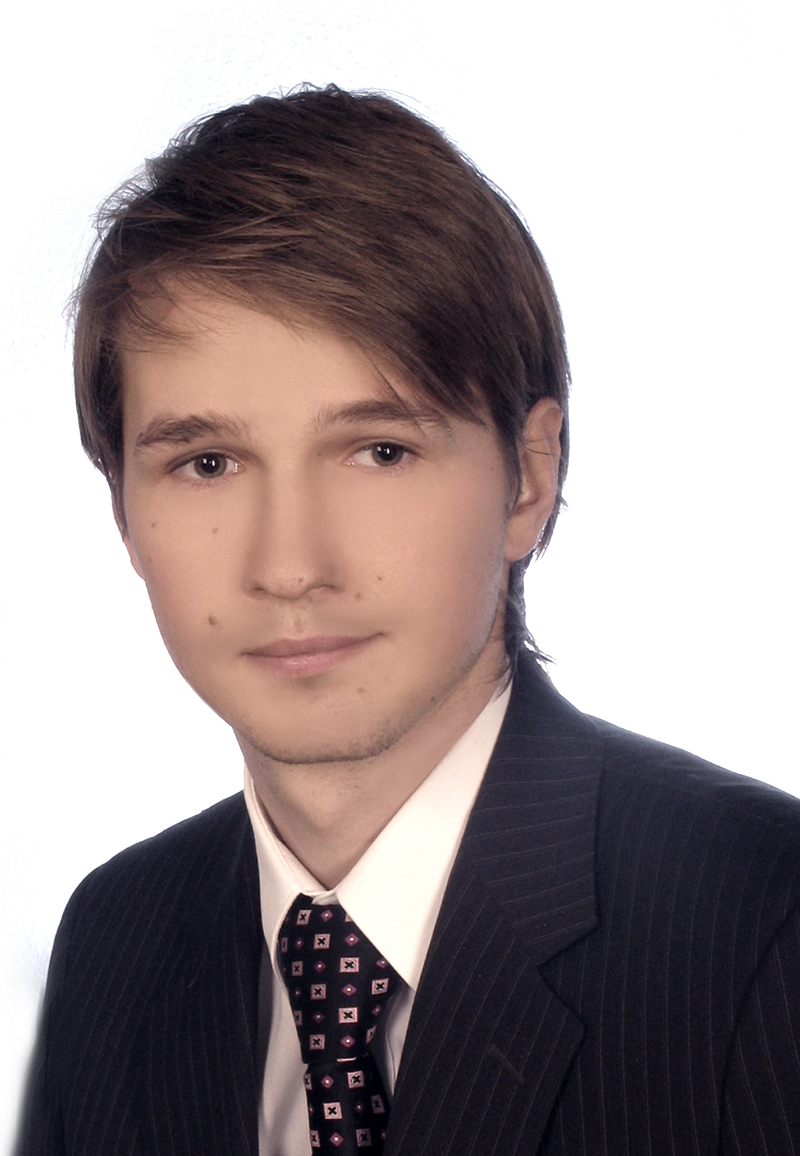
\includegraphics[height=6.5cm,width=4.5cm]{img/foto.jpg}
    \end{minipage}
    &
    \begin{minipage}{12cm}
    \begin{flushleft}
    \par\noindent\vspace{1\baselineskip}
    \begin{tabular}[h]{l l}
    {\normalsize\it Specjalność:} & \normalsize Inżynieria Systemów Informacyjnych 
    \end{tabular}
    \par\noindent\vspace{1\baselineskip}
    \begin{tabular}[h]{l l}
    {\normalsize\it Data urodzenia:} & {\normalsize 12 stycznia 1990~r.}
    \end{tabular}
    \par\noindent\vspace{1\baselineskip}
    \begin{tabular}[h]{l l}
    {\normalsize\it Data rozpoczęcia studiów:} & {\normalsize 1 października 2009 r.}
    \end{tabular}
    \par\noindent\vspace{1\baselineskip}
    \end{flushleft}
    \end{minipage}
    \end{tabular}
    \vspace*{1\baselineskip}
    \begin{center}
	{\large\bfseries Życiorys}\par\bigskip
    \end{center}

    \indent
Urodziłem się 12 stycznia 1990 roku w Piotrkowie Trybunalskim. Ukończyłem Szkołę Podstawową
nr 33, Gimnazjum nr 11 oraz Liceum Ogólnokształcące im. Jana Kochanowskiego w Warszawie, gdzie
uczęszczałem do klasy o profilu matematyczno--fizyczno--informatycznym.
W październiku 2009 roku rozpocząłem studia na Wydziale Elektroniki i Technik Informacyjnych
Politechniki Warszawskiej na kierunku Informatyka. W lutym 2013 roku uzyskałem
tytuł inżyniera.

    \par
    \vspace{2\baselineskip}
    \hfill\parbox{15em}{{\small\dotfill}\\[-.3ex]
    \centerline{\footnotesize podpis studenta}}\par
    \vspace{3\baselineskip}
    \begin{center}
 	{\large\bfseries Egzamin dyplomowy} \par\bigskip\bigskip
    \end{center}
    \par\noindent\vspace{1.5\baselineskip}
    Złożył egzamin dyplomowy w dn. \dotfill
    \par\noindent\vspace{1.5\baselineskip}
    Z wynikiem \dotfill
    \par\noindent\vspace{1.5\baselineskip}
    Ogólny wynik studiów \dotfill
    \par\noindent\vspace{1.5\baselineskip}
    Dodatkowe wnioski i uwagi Komisji \dotfill

  
    % Streszczenie
    \newpage\thispagestyle{empty}
    \vspace*{2\baselineskip}
    \begin{center}
	{\large\bfseries Streszczenie}\par\bigskip
    \end{center}

    {\itshape
W pracy porównano znane algorytmy ewolucji różnicowej DE/rand oraz DE/best z nową odmianą DE/mid.
W części teoretycznej wyprowadzono parametry skalujące dla wszystkich algorytmów. W części praktycznej
przeprowadzono szereg eksperymentów. W wielu wymiarach,
DE/mid/1 okazał się zdecydowanie najlepszy.}
    \vspace*{1\baselineskip}

    \noindent{\bf Słowa kluczowe}: {\itshape ewolucja różnicowa, algorytm ewolucyjny, genetyczny, optymalizacja globalna}
    \par
    \vspace{4\baselineskip}
    \begin{center}
	{\large\bfseries Abstract}\par\bigskip
    \end{center}
    \noindent{\bf Title}: {\itshape DE/mid -- new variant of differential evolution algorithm using the midpoint of the population}\par
    \vspace*{1\baselineskip}
    {\itshape
    This thesis describes \ldots}
    \vspace*{1\baselineskip}

    \noindent{\bf Key words}: {\itshape differential evolution, evolutionary, genetic algorithm, global optimization
}

\end{titlepage}